%!TEX root = ../Technische Dynamik.tex

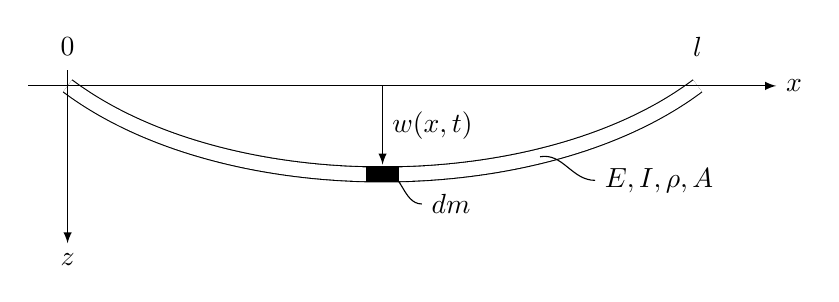
\begin{tikzpicture}[>=latex]
\draw[double distance=5pt] (0,0) .. controls (2,-1.5) and (6,-1.5) .. (8,0);
\draw[fill] (3.8,-1.21) rectangle (4.2,-1.03);
\draw (4,-1.1) to[in=180,out=10] (4.5,-1.5) node[right] {$dm$};
\draw (6,-0.9) to[in=180,out=10] (6.7,-1.2) node[right] {$E,I,\rho,A$};
\draw[->] (4,0) -- node[right] {$w(x,t)$} (4,-1);

\draw[->] (-0.5,0) -- (9,0) node[right]{$x$};
\node at (0,0.5) {$0$};
\node at (8,0.5) {$l$};
\draw[->] (0,0.2) -- (0,-2) node[below]{$z$};
\end{tikzpicture}